\documentclass[journal,compsoc]{IEEEtran}\newcommand{\journal}{true}
%\documentclass[conference]{IEEEtran}\newcommand{\journal}{false}
\ifCLASSOPTIONcompsoc
  % IEEE Computer Society needs nocompress option
  % requires cite.sty v4.0 or later (November 2003)
  \usepackage[nocompress]{cite}
\else
  % normal IEEE
   \usepackage{cite}
\fi

%\providecommand{\tabularnewline}{\\}

\usepackage{indentfirst}

%%--------------------Colocados por minha vontade própria-----------------------
\usepackage{marvosym}
\usepackage[utf8x]{inputenc}
\usepackage[english,brazil]{babel}	
\usepackage[T1]{fontenc}
\usepackage{wasysym}				% setas
\usepackage{picinpar}				% figuras onde eu quero, problemas com referencias
\usepackage{sidecap}				% legenda ao lado da figura
\usepackage[small,bf]{caption}
\usepackage{lipsum}					% Pra encher linguiça
\usepackage{ifthen}
\setcounter{secnumdepth}{6}
\setcounter{tocdepth}{6}

%\usepackage{fancyhdr}
%\lhead{O que quero no cabeçalho parte esquerda}
%\chead{O que quero no cabeçalho parte central}
%\rhead{O que quero no cabeçalho parte direita}
%\lfoot{O que quero no rodapé parte esquerda}
%\cfoot{O que quero no rodapé parte central}
%\rfoot{O que quero no rodapé parte direita}

\input nomes

\usepackage{verbatim}
\usepackage{lmodern}
\usepackage{emp}
\ifx\pdftexversion\undefined
\usepackage[dvips]{graphicx}
\else
\usepackage[pdftex]{graphicx}
\DeclareGraphicsRule{*}{mps}{*}{}
\fi

%%------------------------------------------------------------------------------
%%	Resolveu o problema de a linguagem não estar declarada
\makeatletter
\def\markboth#1#2{\def\leftmark{\@IEEEcompsoconly{\sffamily}\MakeUppercase{\protect#1}}%
\def\rightmark{\@IEEEcompsoconly{\sffamily}\MakeUppercase{\protect#2}}}
\makeatother
%%------------------------------------------------------------------------------
%%----------------Para inclusão de algoritmos em C/C++/Assembly---------------------------
\usepackage{listings}
%\lstnewenvironment{C}
\lstset{%
%inputencoding=utf8,
extendedchars=true,
showstringspaces=false,
language=C,							%linguagem
numbers=left,						%posição dos números
stepnumber=1,						%frequencia de aparição dos números
numbersep=0.5pt,
tabsize=4,
commentstyle=\color{blue},
stringstyle=\color{purple},         % string literal style
%title=\lstname,
basicstyle=\scriptsize\ttfamily}

% Inclua o source com: \lstinputlisting[language=C]{src/src.c}

\lstdefinelanguage{MSP430}
{ %% Se estiver faltando alguma palavra reservada, insira ela aqui
morekeywords={RRC,SWPB,RRA,SXT,PUSH,CALL,RETI,JNE,JNZ,JEQ,
Z,JNC,JLO,JC,JHS,JN,JGE,JL,JMP,NOP,POP,BR,
RET,CLRC,SETC,CLRZ,SETZ,CLRN,SETN,DINT,EINT,
RLA,RLC,ADD,ADDC,INV,XOR,CLR,MOV,TST,CMP,DEC,
SUB,SUBC,DECD,INC,INCD,SBC,MOV,DADD,BIT,
BIC,BIS,XOR,AND,MOV.B,MOV.W},
sensitive=false,
morecomment=[l]{//},
morecomment=[l]{;},
morecomment=[s]{/*}{*/},
}
% Inclua o source com: \lstinputlisting[language=MSP430]{src/src.asm}


%
%%------------------------------------------------------------------------------
%%---------------------Includes importantes para suporte------------------------
\input link							% Para verificar links de citações e outras configurações
%%------------------------------------------------------------------------------
%%------------------------------------------------------------------------------



% *** GRAPHICS RELATED PACKAGES ***
%

\ifCLASSINFOpdf
\usepackage{tikz}
\usepackage{prerex}
\usepackage{helvet}
\usetikzlibrary{positioning,shapes,shadows,arrows}
% \usepackage{tikzgraphicx}
%  \usepackage[pdftex]{graphicx}  
%  \pdfcompresslevel=1
  % declare the path(s) where your graphic files are
  % \graphicspath{{../pdf/}{../jpeg/}}
  % and their extensions so you won't have to specify these with
  % every instance of \includegraphics
  % \DeclareGraphicsExtensions{.pdf,.jpeg,.png}
\else
  \usepackage[dvips]{graphicx}
  % declare the path(s) where your graphic files are
  % \graphicspath{{../eps/}}
  % and their extensions so you won't have to specify these with
  % every instance of \includegraphics
  % \DeclareGraphicsExtensions{.eps}
\fi
\pdfcompresslevel=9



% *** ALIGNMENT PACKAGES ***
%
\usepackage{array}
% Frank Mittelbach's and David Carlisle's array.sty patches and improves
% the standard LaTeX2e array and tabular environments to provide better
% appearance and additional user controls. As the default LaTeX2e table
% generation code is lacking to the point of almost being broken with
% respect to the quality of the end results, all users are strongly
% advised to use an enhanced (at the very least that provided by array.sty)
% set of table tools. array.sty is already installed on most systems. The
% latest version and documentation can be obtained at:
% http://www.ctan.org/tex-archive/macros/latex/required/tools/


%\usepackage{mdwmath}
%\usepackage{mdwtab}
% Also highly recommended is Mark Wooding's extremely powerful MDW tools,
% especially mdwmath.sty and mdwtab.sty which are used to format equations
% and tables, respectively. The MDWtools set is already installed on most
% LaTeX systems. The lastest version and documentation is available at:
% http://www.ctan.org/tex-archive/macros/latex/contrib/mdwtools/


% IEEEtran contains the IEEEeqnarray family of commands that can be used to
% generate multiline equations as well as matrices, tables, etc., of high
% quality.


\usepackage{eqparbox}
% Also of notable interest is Scott Pakin's eqparbox package for creating
% (automatically sized) equal width boxes - aka "natural width parboxes".
% Available at:
% http://www.ctan.org/tex-archive/macros/latex/contrib/eqparbox/





% *** SUBFIGURE PACKAGES ***
%\ifCLASSOPTIONcompsoc
\usepackage[tight,normalsize,sf,SF]{subfigure}
%\else
%\usepackage[tight,footnotesize]{subfigure}
%\fi
% subfigure.sty was written by Steven Douglas Cochran. This package makes it
% easy to put subfigures in your figures. e.g., "Figure 1a and 1b". For IEEE
% work, it is a good idea to load it with the tight package option to reduce
% the amount of white space around the subfigures. Computer Society papers
% use a larger font and \sffamily font for their captions, hence the
% additional options needed under compsoc mode. subfigure.sty is already
% installed on most LaTeX systems. The latest version and documentation can
% be obtained at:
% http://www.ctan.org/tex-archive/obsolete/macros/latex/contrib/subfigure/
% subfigure.sty has been superceeded by subfig.sty.




% *** FLOAT PACKAGES ***
%
\usepackage{float}
\usepackage{fixltx2e}
% http://www.ctan.org/tex-archive/macros/latex/base/


%\usepackage{stfloats}
% stfloats.sty was written by Sigitas Tolusis. This package gives LaTeX2e
% the ability to do double column floats at the bottom of the page as well
% as the top. (e.g., "\begin{figure*}[!b]" is not normally possible in
% LaTeX2e). It also provides a command:
%\fnbelowfloat
% to enable the placement of footnotes below bottom floats (the standard
% LaTeX2e kernel puts them above bottom floats). This is an invasive package
% which rewrites many portions of the LaTeX2e float routines. It may not work
% with other packages that modify the LaTeX2e float routines. The latest
% version and documentation can be obtained at:
% http://www.ctan.org/tex-archive/macros/latex/contrib/sttools/
% Documentation is contained in the stfloats.sty comments as well as in the
% presfull.pdf file. Do not use the stfloats baselinefloat ability as IEEE
% does not allow \baselineskip to stretch. Authors submitting work to the
% IEEE should note that IEEE rarely uses double column equations and
% that authors should try to avoid such use. Do not be tempted to use the
% cuted.sty or midfloat.sty packages (also by Sigitas Tolusis) as IEEE does
% not format its papers in such ways.




% *** PDF, URL AND HYPERLINK PACKAGES ***
%
\usepackage{url}
% http://www.ctan.org/tex-archive/macros/latex/contrib/misc/
% 
% \url{my_url_here}.




% *** Do not adjust lengths that control margins, column widths, etc. ***
% *** Do not use packages that alter fonts (such as pslatex).         ***
% There should be no need to do such things with IEEEtran.cls V1.6 and later.
% (Unless specifically asked to do so by the journal or conference you plan
% to submit to, of course. )


% correct bad hyphenation here
\hyphenation{op-tical net-works semi-conduc-tor}

\begin{document}
	\title{%
\includegraphics[width=18cm]{./fts/cap.png}\\
	\hell\\\ver}
	\author{
%--------------------------------Nomes------------------------------------------
%		\hyperref[luiz]{Luiz Fernando Gomes de Oliveira},~\IEEEmembership{10/46969} 
%		\\\hyperref[panda]{Helbert de Oliveira Coelho Junior},~\IEEEmembership{10/45253}
\ifthenelse{\equal{\journal}{true}}{
\allnames\\
}{
%\thanks{Revisado em \today.}
\IEEEauthorblockN{\luiz}
\IEEEauthorblockA{Matricula: \luizmatricula\\E-mail: \eluiz}
\and
\IEEEauthorblockN{\gust}
\IEEEauthorblockA{Matricula: \gustmatricula\\E-mail: \egust}
\and
\IEEEauthorblockN{\fay}
\IEEEauthorblockA{Matricula: \faymatricula\\E-mail: \efay}
}}

%--------------------------O titulo é inserido aqui!----------------------------
%	\selectlanguage{english}  %seleciona o idioma em inglês [para mater os termos abstract e o thanks em inglês]
	\markboth{Universidade de Bras\'ilia - Campus Gama - FGA, \entrega}%
%{	\begin{figure*}
%    	\includegraphics[width=\textwidth]{./fts/unb.jpg}
%	\end{figure*}
%}
	{Shell \MakeLowercase{\textit{et al.}}: \ver}
%-------------------------------------------------------------------------------

	\IEEEcompsoctitleabstractindextext{%
	\begin{abstract}
		% objetivo do experimento
% resumo do procedimento (forma como o experimento foi executado)
% os resultados sucintamente discutidos
% Deve ser feito de preferencia em Inglês
%
%
\selectlanguage{brazil}  %%Desta linha em diante coloque o resumo apenas em português. Nas linhas anteriores, mantenha o texto em inglês.
%
Apresentação do \assunto. Como foram tomadas as decisões e o que ele pode oferecer. Uma descrição breve sobre seus objetos e compilação.
%


	\end{abstract}}
	%%-------------------------------------
%	\begin{IEEEkeywords} %palavras chaves
%		\keyw %,\LaTeX.
%	\end{IEEEkeywords}}
	% make the title area
%\onecolumn		%Conferir se pode ser feito em duas colunas

	\maketitle

	\IEEEdisplaynotcompsoctitleabstractindextext
	\IEEEpeerreviewmaketitle

	\selectlanguage{brazil}		%voltando para o português.
	%\tableofcontents			% Sumario

	\section{Introdução}\label{intro}
		%Definir, caracterizar e mostrar um breve historico e as utilidades do foco



%Segue um exemplo de como INICIAR o texto. Da segunda palavra em
%diante, escreva normalmente
%	\IEEEPARstart{T}{his} demo file is intended to serve as a ``starter file''
%	for IEEE Computer Society journal papers produced under \LaTeX\ using
%	IEEEtran.cls version 1.7 and later.
%
%	\IEEEPARstart{D}{escrição}, com textos e imagens, da configuração do procedimento e cenário experimental. Explorar técnicas e métodos de medida 
%
\nocite{dsl} %Apresenta a referência, porém não cita no texto
\subsection{Objetivos}\label{obj}

\IEEEPARstart{E}{ste} experimento tem como objetivo descrever um passo a passo de como obter um ambiente básico para as demais aulas. Para isso, precisamos ter uma distribuição contendo os aplicativos fundamentais para o desenvolvimento da matéria de Sistemas Embarcados.
	
\subsection{Introdução Teórica}\label{intro}	
\subsubsection{Damn Small Linux}\label{dsl}
\textit{Damn Small Linux}, ou apenas DSL, é uma distribuição versátil do Linux, tendo o tamanho de cerca de 50mb e ocupando como espaço final na RAM cerca de 128MB. A distribuição foi montada com o intuito de cumprir os seguintes objetivos:
	
%\hfill \today

\subsubsection{Material}\label{mat}
Será usado a versão 4.4.10 do DSL, com o Kernel 2.4.31, em um placa de modelo PCM-9375, munida de um processador AMD Geode™ LX80 e suporte para comunicação USB, RJ-45, RS-232 e saídas de vídeo CRT e TFT LCD. É de opção do aluno apresentar também o experimento em seu computador pessoal ou em algum dos notebooks fornecidos pela universidade na sala.
%\hfill \today
	
\begin{itemize}
	\item PCM-9375
	\item Damn Small Linux (v4.4.10)
	\item Distribuição Linux qualquer para remasterização do DSL
	\item GCC
\end{itemize}	
	





	
	\section{Desenvolvimento}\label{hardsoft}
		% Deve resumir o experimento, os resultados e a discussão (comentários)
% e incluir opiniões do grupo e propostas futuras para o experimento
%Descrição do hardware
%Descrição do software
%\cite{Advpdf}
%\cite{thepdf}
%\cite{dsl}

\subsection{Estruturas}\label{struct}

\subsubsection{Arquitetura}\label{arq}

No intuito de manter o jogo compatível com qualquer sistema operacional, foi decidido centralizar as inclusões de bibliotecas em um único arquivo. Para essa função foi criado o arquivo \textit{"defines.h"}, que é responsável por reconhecer o sistema em que esta sendo compilado e incluir os devidos \textit{headers}.

\begin{lstlisting}[language=C++,title=\textit{defines.h},firstnumber=5,numbers=none]
#if defined (__APPLE__) || defined (MACOSX) /*MAC OS*/
    #include <GLUT/glut.h>
#else
    #ifdef _WIN32                           /* Windows */
    	#define WIN32_LEAN_AND_MEAN
        #include <glee.h>
        #include <gl/gl.h>
		#include <gl/glut.h>
        #include <windows.h>
        #define sleep(x) Sleep(x)
    #else                                   /*Linux*/
    	#include <cstdarg>
    	#include <unistd.h>
        #include <GL/gl.h>
        #include <GL/glut.h>
        #include <GL/glu.h>
        #define Sleep(x) usleep(x<1000000?10000+300*x:x)
    #endif
#endif
\end{lstlisting}

No trecho mostrado acima, podemos ver como o programa reconhece em qual sistema esta sendo compilado e em qual endereço irá procurar pelas bibliotecas. A decisão é tomada de forma bem simples e objetiva, buscando apenas saber se as definições \textbf{MACOSX} ou \textbf{\_WIN32} existem. Com estas duas definições é suficiente para dividir entre os três sistemas operacionais que o programa se propõe a dar suporte. 

Porém este não é o único problema enfrentado quando se trata de um programa multiplataforma, mas também existem as dificuldades com a própria compilação.

Visando isso, foi feito um arquivo \textit{makefile} que procede com teste semelhante ao feito no \textit{defines.h} para verificar em que sistema se encontra e assim efetuar os links corretamente. Um trecho do \textit{makefile} pode ser observado a seguir:

\begin{lstlisting}[language=make,title=\textit{Makefile},firstnumber=8,numbers=none]
UNAME = $(shell uname)
ifeq ($(UNAME),Linux) # Linux OS
	GLFLAGS = -lglut -lglui -lGLU -lGL -lalut -lopenal
	else
	ifeq ($(UNAME),Darwin) # MAC OS X
		GLFLAGS = -framework OpenGL -framework GLUT
	else #Windows
		GLFLAGS = -lopengl32 -lglu32 -lglut32 -lglee -lalut
	endif
endif
\end{lstlisting}

É valido aproveitar a oportunidade para frisar no trecho mostrado acima do \textit{makefile} a inclusão das flags \textit{-lalut -lopenal} para inclusão de áudio no programa.

\subsubsection{Execução}\label{exe}

\paragraph{\textbf{Windows}}

O programa foi desenvolvido com auxilio da IDE \textit{CodeBlocks}\footnote{Acesse \url{http://www.codeblocks.org/} para maiores informações sobre a IDE.}. Assim, para gerar o executável na plataforma, basta abrir o arquivo \textit{Projeto - Labirinto.cbp} no \textit{CodeBlocks} e mandar compilar/construir o projeto. Na própria IDE haverá meios de executar o arquivo de saída, porém na pasta do projeto será possível localizar também o arquivo \textit{*.exe}.

\paragraph{\textbf{Linux}}

Para se construir o programa na plataforma Linux, é necessário ter algumas bibliotecas instaladas no sistema. Dentre elas é valido destacar as do OpenGL e de áudio (\textit{Alut} e \textit{Openal}). Na pasta onde se encontra os arquivos fontes, é possível localizar o arquivo \textit{makefile}. No terminal, basta executar o comando \textbf{make run} no diretorio contendo o arquivo \textit{makefile} para compilar os arquivos e inicializar o programa corretamente. Caso alguma das bibliotecas necessárias não estejam instaladas, será observado a lista de \textit{warnings/errors}, orientando qual biblioteca deve de ser instalada. É valido lembrar que para instalar as bibliotecas para este fim na plataforma Linux, deve-se buscar pelos nomes com o sufixo \textit{-dev}, garantindo assim que serão instalados os arquivos necessários. A compilação será feita de forma silenciosa e se não tiver problemas, apresentará uma saída semelhante a:

\begin{lstlisting}[language=bash,title=\textit{Saída do terminal - Linux},numbers=none]
$ make run
System: Linux OS
compiling...ok
Running...
\end{lstlisting}

\paragraph{\textbf{Mac OS}}

Semelhante aos passos no sistema Linux, o usuário terá que executar o comando \textbf{make run} no diretorio contendo o arquivo \textit{makefile} para compilar os arquivos e inicializar o programa corretamente. Se a compilação ocorrer corretamente, a saída deverá ser semelhante a:

\begin{lstlisting}[language=bash,title=\textit{Saída do terminal - Mac OS},numbers=none]
$ make run
System: Darwin
compiling...ok
Running...
\end{lstlisting}


\subsubsection{Artefatos}\label{artefatos}

\paragraph{\textbf{Arquivos}}

Arquivos utilizados na construção do programa\footnote{Atualizado em 7 de Junho de 2012}:\\

\begin{itemize}
	\item button.cpp
	\item camera.h
	\item entidade.cpp
	\item eventos.h 
	\item gamemanager.cpp  
	\item map.h        
	\item minimap.h   
	\item soundAL.cpp  
	\item text.h             
	\item tile.cpp   
	\item vetor.h
	\item button.h    
	\item defines.cpp  
	\item entidade.h    
	\item framerate.cpp  
	\item gamemanager.h    
	\item maze.h       
	\item player.cpp  
	\item soundAL.h    
	\item textureloader.cpp  
	\item tile.h
	\item camera.cpp  
	\item defines.h    
	\item eventos.cpp   
	\item framerate.h    
	\item map.cpp          
	\item minimap.cpp  
	\item player.h    
	\item text.cpp     
	\item textureloader.h    
	\item vetor3d.h
\end{itemize}

\paragraph{\textbf{README}}

O arquivo README pode ser localizado dentre os arquivos fontes, em \ref{README}.

\subsubsection{Problemas Técnicos}\label{problens}

No decorrer da construção do programa a maior dificuldade foi ...

\textbf{TODO :\\ VERIFICAR ISSO}

%-----------------------------------------------------------------------------------------------------------------
\textbf{SEGUNDO a professora:\\}
Na seção desenvolvimento deve ser respondidas as seguintes perguntas:
 
	\begin{itemize}
	 	\item Como os pontos relacionados à disciplina foram abordados no problema? Quais as lições aprendidas? Quais as principais dificuldades?
	 	\item Quais elementos teóricos abordado na disciplina foram implementados no programa?
	 	\item Quais adaptações, extensões, bibliotecas externas, foram necessários para a solução do problema?
	 	\item Caso use parte de códigos disponibilizados na Web, colocar referência \footnote{A home-page de onde tirei
este material:\url{http://en.wikibooks.org/wiki/LaTeX}.Estou formatando para \LaTeX apenas para os estudantes irem se orientando de como e o quê escrever.Assim, me isento de responsabilidade sobre o conteúdo deste texto. Dúvidas: carla(rocha.carla@gmail.com)}
	\end{itemize}
	
	As Figuras são simplesmente inseridas como mostrado na Fig. \ref{Fig1}
	
\begin{figure}[ht]
  \centering
  %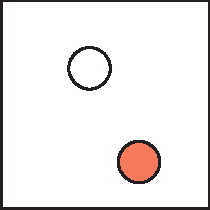
\includegraphics[width=5cm]{figs/samplefigure}
   \caption{Arquitetura do Programa.}
  \label{Fig1}
\end{figure}
 
\subsection{Artefatos}
\label{SebSec:Artefatos}
Os artefatos entregues devem ser documentados no relatório:
\begin{itemize}
\item Arquivos contidos no programa. Lista dos nomes dos arquivos, assim como a extensão dos arquivo
\item Aquivo README, com instruções de uso do software desenvolvido e necessidades técnicas para a execução do programa
\item Arquivos de entrada/saída, caso necessário.
\end{itemize}


	
	\section{Caso de Teste}\label{resultados}
		
Nessa seção deve ser apresentado pelo menos um exemplo de caso de teste. Se não for especificado na descrição do problema, ela deve definida, explicada e ilustrada pelos autores.

	
	\section{Conclusão}\label{conclusion}
		%Deve conter a tabela verdade obtida em laboratorio comentada
%(principalmente nos estados ambíguos)
%Deve apresentar também as dificuldades encontradas no experimento

%Apresentação dos resultados referentes à confecção do modelo em estudo e medidas realizadas, 
%\begin{SCfigure}[1][h] %%Cuidado..ela não se mantem no lugar
%  \centering
%  \includegraphics[width=4cm]{./fts/unb}
%  \caption{Legenda da figura \ref{caption1}. Coloca qualquer coisa.}
%  \label{caption1}
%\end{SCfigure}
%em forma de texto, tabelas e gráficos, como visto na figura \ref{caption} ou na figura \ref{caption1}. Também pode ser incluida nos anexos, como a figura \ref{unb}.
%\lipsum[2]

\subsection{Dificuldades encontradas}\label{dificuldades}

\begin{itemize}
	\item Dificuldades em discubrir o modo com que o glut atrubui as funções e gerencia os eventos.
	\item Dificuldades em tornar o jogo jogável por multiplataformas; especificamente no tratamento de sons.
	\item Dificuldade em imprimir objetos 2d por cima do cenario 3d (minimap)
\end{itemize}

\subsection{Sugestões}\label{sugest}

\begin{itemize}
	\item Multiplayer para 2 jogadores Alternados.
	\item Registro de nome para usuarios que concluirem um nível com sua respectiva potuação.
\end{itemize}

%\subsubsection{Pontos relevantes abortados}\label{relevantes} %que seriam uteis na prática e a relevância de tais conceitos (Exemplo de aplicações que tais conceitos seriam úteis). Com citações  se necessário.




	\ifCLASSOPTIONcaptionsoff
	  \newpage
	\fi

	\bibliographystyle{IEEEtran}%{abnt-num}%{ieeetr}%{abnt-alf}
	\bibliography{bibliography}		% expects file "bibliography.bib" 

	%\else
	%\begin{thebibliography}{6} 
	%O Número implica na quantidade MÁXIMA de itens que pode haver de bibliografias.
	%Altere-o se tiver usado mais que duas fontes.

	%\bibitem{IEEEhowto:kopka}
	%H.~Kopka and P.~W. Daly, \emph{A Guide to \LaTeX}, 3rd~ed.\hskip 1em plus
	%  0.5em minus 0.4em\relax Harlow, England: Addison-Wesley, 1999.

	%\bibitem{Wakerly}
	%John F. Wakerly, \emph{Digital Design: Principles and Practices}, 3rd~ed.
	%	\hskip 1em plus 0.5em minus 0.4em\relax Prentice Hall, 1999.

	%\bibitem{zelenovsky}
	%Mendonça A. e Zelenovsky R., \emph{Eletrônica Digital: Curso Prático e Exercícios}, MZ Editora, Brasil, 2004.
	%Contemporary Logic Design - Katz R. H., First Edition, 1993.	

	%\end{thebibliography}
	%\fi

	\begin{IEEEbiography}[{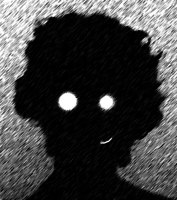
\includegraphics[width=1in,height=1.25in,clip,keepaspectratio]{./fts/luiz}}]{\luiz}\label{luizbio}
	
	Matricula: \luizmatricula
	
	E-mail: \eluiz
	\end{IEEEbiography}
	
	\begin{IEEEbiography}[{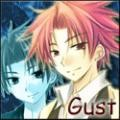
\includegraphics[width=1in,height=1.25in,clip,keepaspectratio]{./fts/gust}}]{\gust}\label{gustbio}
	
	Matricula: \gustmatricula
	
	E-mail: \egust
	\end{IEEEbiography}
	
	\begin{IEEEbiography}[{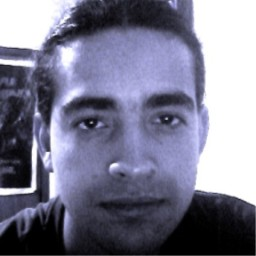
\includegraphics[width=1in,height=1.25in,clip,keepaspectratio]{./fts/fay}}]{\fay}\label{faybio}
	
	Matricula: \faymatricula
	
	E-mail: \efay
	\end{IEEEbiography}

%\newpage
\onecolumn
\appendices
		\section{Códigos Fontes}\label{src}

%------------------------------------------------------------------------------%		
% Anexar source main.c com link
%\hypertarget{main}{
%\lstinputlisting[language=C,texcl=true]{../main.c} }
%anexar source main.c sem link
%\lstinputlisting[language=C]{../main.c}
%------------------------------------------------------------------------------%		
%\cite{ti_exemplos}
%\tableofcontents %Índice de conteúdos
%\listoftables %Lista de tabelas
%\listoffigures %Lista de figuras
%------------------------------------------------------------------------------%		
\subsection{Headers}\label{.h}

\subsubsection{Camera}
\lstinputlisting[language=C++]{../../trunk/camera.h}
\subsubsection{Entidade}
\lstinputlisting[language=C++]{../../trunk/entidade.h}
\subsubsection{Framerate}
\lstinputlisting[language=C++]{../../trunk/framerate.h}
\subsubsection{Map}
\lstinputlisting[language=C++]{../../trunk/map.h}
\subsubsection{Texture Loader}
\lstinputlisting[language=C++]{../../trunk/textureloader.h}
\subsubsection{Defines}
\lstinputlisting[language=C++]{../../trunk/defines.h}
\subsubsection{Eventos}
\lstinputlisting[language=C++]{../../trunk/eventos.h}
\subsubsection{Text}
\lstinputlisting[language=C++]{../../trunk/text.h}

\subsection{Sources}\label{.cpp}

\subsubsection{Camera}
\lstinputlisting[language=C++]{../../trunk/camera.cpp}
\subsubsection{Entidade}
\lstinputlisting[language=C++]{../../trunk/entidade.cpp}
\subsubsection{Framerate}
\lstinputlisting[language=C++]{../../trunk/framerate.cpp}
\subsubsection{Map}
\lstinputlisting[language=C++]{../../trunk/map.cpp}
\subsubsection{Texture Loader}
\lstinputlisting[language=C++]{../../trunk/textureloader.cpp}
\subsubsection{Defines}
\lstinputlisting[language=C++]{../../trunk/defines.cpp}
\subsubsection{Eventos}
\lstinputlisting[language=C++]{../../trunk/eventos.cpp}
\subsubsection{Game Maneger}
\lstinputlisting[language=C++]{../../trunk/gamemanager.cpp}
\subsubsection{Text}
\lstinputlisting[language=C++]{../../trunk/text.cpp}
\subsubsection{Title}
\lstinputlisting[language=C++]{../../trunk/tile.cpp}
\subsubsection{Makefile}
\lstinputlisting[language=make]{../../trunk/Makefile}
\subsubsection{README}\label{README}
\lstinputlisting[language=make,texcl=true,numbers=none]{../../trunk/README}

\onecolumn
\section{Anexos}\label{anexo}

\begin{figure}[h]
	\centering
	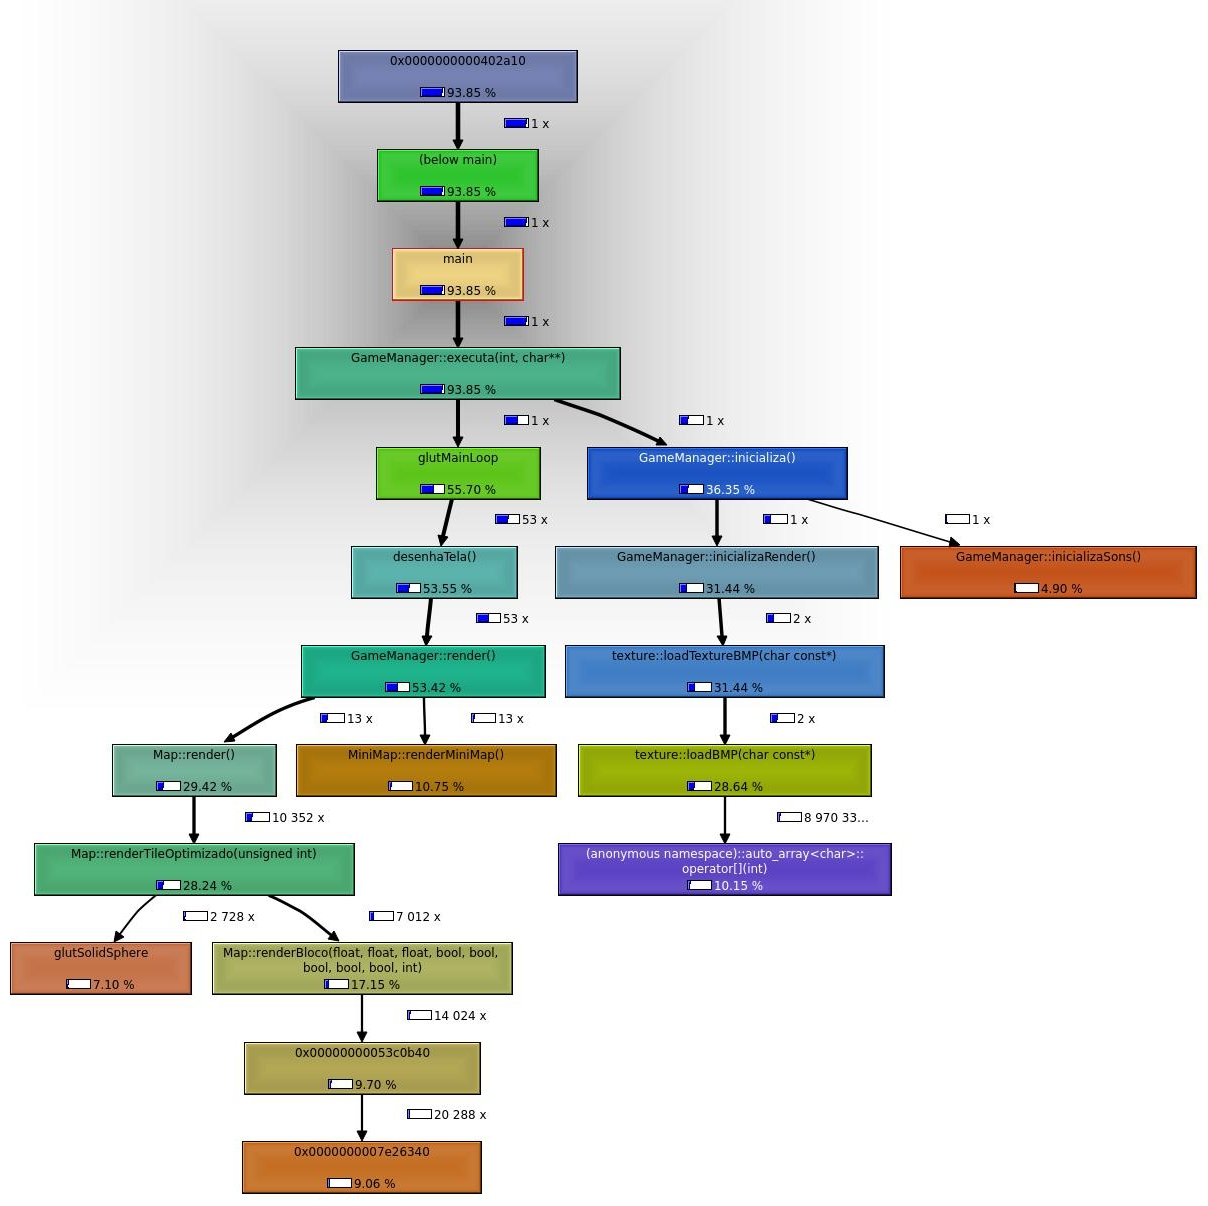
\includegraphics [scale=0.5,angle=0,keepaspectratio=true]{./fts/callgrind/img3}
	\caption{Saída gerada pelo Valgrind}
	\label{valgrind}
\end{figure}

%-------------------------------------------------------------------------

% End of code
% End of code


%Inclusão de Figuras
%--------------------Figura logo da UnB----------------------------------------%
%\begin{figure}[h]
%	\centering
%	\includegraphics [scale=1,angle=0,keepaspectratio=true]{./fts/unb}
%	\caption{Logo da UnB}
%	\label{unb}
%\end{figure}
%--------------------Figura logo da UnB----------------------------------------%
%\begin{SCfigure}[1][h] %%Cuidado..ela não se mantem no lugar
%  \centering
%  \includegraphics[width=4cm]{./fts/unb}
%  \caption{Logo da UnB.}
%  \label{unb1}
%\end{SCfigure}


%\begin{multicols}{4}
%\tikzstyle{cloud} = [draw, ellipse,fill=red!20, node distance=3cm,
%    minimum height=2em]
%\tikzstyle{phanton} = []   
%\tikzstyle{line} = [->,bend left] %[draw, -latex']
%\tikzstyle{arrow} = [loop above]
%
%\begin{center}
%\begin{tikzpicture}[node distance = 2cm]
%	\tiny\ttfamily
%	%-- Estados
%	\node [cloud] (E0) at(0,2) {E0};
%	\node [cloud] (E1) at(2,1) {E1};
%	\node [cloud] (E2) at(2,-1) {E2};
%	\node [cloud] (E3) at(0,-2) {E3};
%	\node [cloud] (E4) at(-2,-1) {E4};
%	\node [cloud] (E5) at(-2,1) {E5};
%	%-- setas
%	\path (E0) edge [line] (E1);
%	\path (E1) edge [line] (E2);
%	\path (E2) edge [line] (E3);
%	\path (E3) edge [line] (E4);
%	\path (E4) edge [line] (E5);
%	\path (E5) edge [line] (E0);
%	%-- Desvios
%	\path (E0) edge [draw,loop above] node{controle1=1} (E0);
%	\path (E3) edge [draw,loop below] node{controle2=1} (E3);
%	\path (E2) edge [bend right,->]  node[anchor=east]{controle1=1\&\&controle2=0} (E0);
%	\path (E5) edge [bend right,->]  node[anchor=west]{controle1=0\&\&controle2=1} (E3);
%\end{tikzpicture}
%\\\hypertarget{diagrama}{Diagrama de Estados}
%\end{center}


%\end{multicols}


%\setcounter{diagheight}{50}
%\begin{chart}
%\reqfullcourse 50,45:{ }{GameManager::Loop}{gamemanager.cpp}
%\reqhalfcourse 30,30:{2813}{Loop()}{MWF 8:30}
%  \prereq 50,45,30,30:
%
%\reqhalfcourse 20,20:{2813}{testColisao()}{MWF 8:30}
%  \prereq 30,30,20,20:
%\end{chart}

% Define block styles
\tikzstyle{decision} = [diamond, draw, fill=blue!20, 
    text width=4.5em, text badly centered, node distance=3cm, inner sep=0pt]
\tikzstyle{block} = [rectangle, draw, fill=blue!20, 
    text width=5em, text centered, rounded corners, minimum height=4em]
\tikzstyle{line} = [draw, -latex']
\tikzstyle{cloud} = [draw, ellipse,fill=red!20, node distance=3cm,
    minimum height=2em]

%\begin{figure}
%    \centering
%\begin{tikzpicture}[node distance = 2cm, auto]
%	
%	\node [block] (init) {Manager\\executa()};
%	
%\end{tikzpicture}
%\caption{Diagrama de Fluxo}
%\end{figure}

%-------------------------------------------------------------------------------

%\begin{figure}
%    \centering
%\begin{tikzpicture}[node distance = 2cm, auto]
%    % Place nodes
%    \node [block] (init) {initialize model};
%    \node [cloud, left of=init] (expert) {expert};
%    \node [cloud, right of=init] (system) {system};
%    \node [block, below of=init] (identify) {identify candidate models};
%    \node [block, below of=identify] (evaluate) {evaluate candidate models};
%    \node [block, left of=evaluate, node distance=3cm] (update) {update model};
%    \node [decision, below of=evaluate] (decide) {is best candidate better?};
%    \node [block, below of=decide, node distance=3cm] (stop) {stop};
%    % Draw edges
%    \path [line] (init) -- (identify);
%    \path [line] (identify) -- (evaluate);
%    \path [line] (evaluate) -- (decide);
%    \path [line] (decide) -| node [near start] {yes} (update);
%    \path [line] (update) |- (identify);
%    \path [line] (decide) -- node {no}(stop);
%    \path [line,dashed] (expert) -- (init);
%    \path [line,dashed] (system) -- (init);
%    \path [line,dashed] (system) |- (evaluate);
%\end{tikzpicture}
%\caption{Diagrama de Fluxo}
%\end{figure}

		
		
\end{document}


